\documentclass[12pt]{article}

\usepackage{
amssymb,
amsmath,
amsfonts,
eurosym,
geometry,
ulem,
graphicx,
caption,
color,
setspace,
sectsty,
comment,
footmisc,
caption,
pdflscape,
subfigure,
array,
natbib,
longtable,
booktabs}
\usepackage[colorlinks=true, allcolors=blue]{hyperref}
\usepackage[flushleft]{threeparttable}
\usepackage{fontspec}
 
\setmainfont{Times New Roman}


\normalem

\onehalfspacing
\newtheorem{theorem}{Theorem}
\newtheorem{corollary}[theorem]{Corollary}
\newtheorem{proposition}{Proposition}
\newenvironment{proof}[1][Proof]{\noindent\textbf{#1.} }{\ \rule{0.5em}{0.5em}}

\newtheorem{hyp}{Hypothesis}
\newtheorem{subhyp}{Hypothesis}[hyp]
\renewcommand{\thesubhyp}{\thehyp\alph{subhyp}}

\newcommand{\red}[1]{{\color{red} #1}}
\newcommand{\blue}[1]{{\color{blue} #1}}

\newcolumntype{L}[1]{>{\raggedright\let\newline\\arraybackslash\hspace{0pt}}m{#1}}
\newcolumntype{C}[1]{>{\centering\let\newline\\arraybackslash\hspace{0pt}}m{#1}}
\newcolumntype{R}[1]{>{\raggedleft\let\newline\\arraybackslash\hspace{0pt}}m{#1}}

\makeatletter
\def\@fnsymbol#1{\ensuremath{\ifcase#1\or \dagger\or \ddagger\or
   \mathsection\or \mathparagraph\or \|\or **\or \dagger\dagger
   \or \ddagger\ddagger \else\@ctrerr\fi}}
\makeatother

\geometry{left=1.5in,right=1.5in,top=1.5in,bottom=1.5in}

\begin{document}

\begin{titlepage}
\title{The effects of mother tongue instruction on employment: Evidence from Ethiopia}
\author{Teferi Mergo\thanks{University of Waterloo. Email \href{tmergo@uwaterloo.ca}{tmergo@uwaterloo.ca} (corresponding author)} \\ 
University of Waterloo 
    \and Lemi Daba\thanks{University of Maryland. Email: \href{ldaba@umd.edu}{ldaba@umd.edu} } \\
    University of Maryland}    
\date{}
\maketitle 

\begin{center}
    \textbf{Abstract}
\end{center}
%\phantomsection % required if using hyperref
%\addcontentsline{toc}{section}{\abstractname}
\doublespacing

Research on the impacts of mother tongue instruction (MTI) on labor market outcomes is limited. MTI improved salary employment in Ethiopia, without any effect on wage employment. The positive effect of MTI on salary employment is consistent with the prevailing ethno-linguistic federalism in the country and a suggestive evidence in this study that cognitive ability increased with MTI. Being from a region with a historically dominant language does not confer advantages in the labor market. MTI increases employment if it is complemented by appropriate institutional and policy measures.\\

\vspace{0in}
\noindent\textbf{Keywords:} Mother Tongue Instruction; Cognitive Ability; Employment;\\
\vspace{-.2in}\\
\noindent\textbf{JEL Codes:} I25, I28, J21, J24, J48\\

\bigskip




\setcounter{page}{0}
\thispagestyle{empty}
\end{titlepage}
\pagebreak \newpage

\doublespacing

\section{Introduction}
\label{section:intro}

In a multilinguistic society with a historically dominant language serving as the lingua franca, it is unclear whether the introduction of mother tongue instruction (MTI) increases employment opportunities.  Links between MTI and success in the labor market are theoretically unclear, nor empirically well-established, although whether MTI contributes to employment outcomes is a topical research question.  

Generally, MTI affects labor market outcomes through its effects on education and proficiency of a prominent language. Several studies document that MTI in early grades improves educational outcomes \citep[e.g.,][]{Walter2012,taylor_estimating_2016}. However, MTI does not necessarily lead to improved education, as the mediating factors can enhance or diminish access to curriculum content and learning \citep{Heugh2007}. The capacity of social groups to make use of their rights, language teaching methodologies, language teaching programs design, and availability of textbooks are some of the factors that determine the efficacy of learning in any language, suggesting that the impact of MTI on education may vary according to the context in which it is implemented. 

MTI may improve education and still result in poor job outcomes if it reduces proficiency in a dominant language. Although it helps to master international languages better at higher levels \citep[e.g.,][]{seid_impact_2019}, MTI can negatively affect employment and earnings by hampering fluency in a dominant language \citep[e.g.,][]{chiswick_endogeneity_2015}. Hence, whether MTI affects employment or not is an empirical research question with important policy implications. 

We test a conjecture that MTI induces differences in employment outcomes through both the education and the prominent-language channels, by exploiting a major policy change as a source of variation in the treatment. After installing ethnic federalism in 1994, Ethiopia introduced MTI in its primary schools, with each state adopting the national policy with different rates of intensity.\footnote{A map of Ethiopia divided into ethnic states is shown in Figure\ref{fig:map}.} Prior to 1994, Amharic was the language of instruction in elementary schools throughout the country, serving both as a source of contestation (for cultural reasons) and as a ladder of upward mobility in the center. Thus, a study based on the institution of MTI in this context may reveal interesting new insights on the relationships between the choice of a language of instruction and the outcomes of employment.  


We instrument variations in MTI intake by the interaction of ethnic identity of students and the MTI policies of the regional states, generating an exogenous IV named Predicted MTI. A review of the MTI adoptation processes in each state reveals that the geographic spread of MTI was randomly determined without the appropriate justifications \citep{Heugh2007}. In states where MTI is used less intensely than was recommended by national policy, for example, policy makers relied on unsubstantiated claims that English would be more beneficial as a medium of instruction in elementary schools \citep{Heugh2007}, although the dissemination and use of English is distinctly and similarly low in all federated states of Ethiopia \citep{gerencheal2019foreign}. 

We conduct two tests that suggest that Predicted MTI is as good as randomly assigned and satisfies the exclusion restriction. First, we show that there are no discernible correlations between employment and predicted MTI in samples where there is no obvious reason for associations between the treatment and employment outcomes. We also compare employment outcomes in states that implemented the MTI policy similarly to check if the treatment effects are driven by unobserved differences in state characteristics, which may lead to variations in demand for formal education and labor market outcomes.

We find that the impact of MTI on employment is mixed (Table \ref{tab:mainreg}).  MTI increased salary employment, but has no discernible effect on wage employment. The increase in salary employment in MTI is consistent with the evidence in Table \ref{tab:rev} that cognitive ability increased with MTI, suggesting that mastery of the dominant language, Amharic, is less important to obtain salaried jobs. 

The finding that the introduction of MTI in Ethiopia has proven to be a double-edged sword in terms of employment generation is reasonable considering the prevailing social infrastructure in the country. Most salaried jobs are in the public sector, where employees have legal rights to work in their native languages. In the private sector, where the mastery of Amharic is still essential to obtain wage employment, the positive effects of the treatment on human capital have been offset by its likely unintended adverse effects on the mastery of the dominant language (Table \ref{tab:rev}). Therefore, MTI increases employment outcomes only if it is complemented with appropriate institutional and policy measures.

These findings do not change when we exclude the Amhara state from the analysis. The magnitudes of MTI's effects on employment and the qualitative conclusions of the study are remarkably similar when the analysis is conducted using the overall sample or only the sample from states with previously suppressed languages, indicating that being from the region with a historically dominant language as such does not confer special advantages in the labor market. 

Our paper contributes to the emerging empirical literature that examines the effects of MTI on labor market outcomes. Studies that have found that MTI improves labor market outcomes link these gains to the positive effects of MTI on education \citep[e.g.,][]{eriksson_does_2014,seid_does_2016,Alidou2006,Walter2012,eriksson_does_2014,taylor_estimating_2016,seid_does_2016,piper_implementing_2016,ramachandran_language_2017,laitin_legacy_2019}, typically through increased participation in schools, reduced grade repetition and dropouts \citep{Benson2000,Benson2005,bender_their_2005} and increased chances of building non-language cognitive skills such as literacy and numeracy \citep{eriksson_does_2014,Trudell2012}.  

%The effectiveness of MTI is highly sensitive to choices of inputs and outcome measures as well as implementation details \citep{kerwin_making_2021}

%In a study conducted in Ethiopia, \citet{chicoine_schooling_2019} asserts that the shift to mother tongue instruction has led to a reduction in schooling and had no impact on literacy, with the negative impact being concentrated in regions that made the switch from an Amharic script to the Roman script. 

MTI has led to negative job outcomes by reducing proficiency in a dominant language \citep[e.g.,][]{angrist_effect_1997}. Having greater proficiency in a dominant language is important for success in the labor market in certain contexts \citep{chiswick_immigrant_2000,chiswick_endogeneity_2015,bleakley_language_2004,munshi_traditional_2006,lang_return_2009,aldashev_language_2009,shastry_human_2012,casale_english_2011,parinduri_effects_2018}, as it improves job search results, productivity on the job, and promotion to higher paying positions \citet{kahn_returns_2019}. %More recently, \citet{parinduri_effects_2018}, using data from Malaysia, have shown that having English as a medium of instruction improves English proficiency and educational attainment, albeit with a weaker link to later labour market outcomes. 
Hence, mother tongue instruction could negatively affect employment outcomes if it adversely affects fluency in a dominant language, although it is unclear what causes the trade-off between learning in mother tongue and mastery of a dominant language. 

%Most of the empirical analysis on the effects of MTI is conducted in contexts where an international language served as a lingua franca \citep[e.g.,][]{eriksson_does_2014,laitin_legacy_2019}. For instance, \citet{eriksson_does_2014} examined the effect of mother tongue vs. English or Afrikaans instruction using the Bantu Education Act of 1955 in South Africa as a natural experiment and finds that increasing MTI from four to six years positively affected wages, literacy, educational attainment, and English speaking skills. \citet{laitin_legacy_2019} conducted a randomized evaluation of a local language schooling program in Cameroon and found that students that were exposed to three years of the local language (Kom) in early grades scored higher in math and English tests than untreated students, who were instructed solely in English. 


%The socio-economic outcomes of shifting from a dominant language (international or domestic) to MTI are mediated through a number of factors, including the degree of people's prior exposure to the dominant language in question \citep{ramachandran_language_2017,laitin_legacy_2019}. 

The majority of existing studies on the effects of MTI are conducted in countries with an international language serving as lingua franca. Our study evaluates the impact of MTI in Ethiopia, where it was introduced as part of a larger strategy to change the character of the Ethiopian state, from a unitary system that had prioritized the assimilation of the diverse population of the country into Amharic speaking citizens, to a federation of self-governing ethnic states with their own official local languages \citep{bulcha_politics_1997,getachew_language_2006}. Arguably, the introduction of MTI was aimed at tackling the inherent contradictions of the Ethiopian state that had prioritized the development of Amharic at the expense of the other local languages. Hence, this study may yield useful insights for policy makers seeking to implement optimal policy solutions to the increasing demands of many linguistic communities around the world to learn and work in their native languages. 

%As \citet{long_bilingual_2009} rightly notes, “language as a medium of instruction confers recognition, status, and often economic benefits (e.g., teaching positions) on speakers of that language ... [and] it is ... a socio-political phenomenon that is implicated in the ongoing competition between social groups for material and symbolic resources.”

Our article is closely related to two recent studies conducted in Ethiopia \cite{seid_mother-tongue_2022} and \cite{chicoine_schooling_2019}, which, due to data constraints, are based on a less rigorous premise that the dominant ethnic language in each regional state is the only language of instruction in each state. Consequently, \cite{seid_mother-tongue_2022} excluded from its analysis all samples from the South due to the state's heterogeneity in terms of ethnicity and found that MTI has positive effects on earnings, and those effects decrease with the duration of exposure to MTI in primary school. Using a similar strategy that excludes ethnic heterogeneity within a region, \citep{chicoine_schooling_2019} examines the impact of MTI on schooling and literacy rates in Ethiopia, finding that the introduction of MTI had led to a reduction in schooling with no impact on literacy, particularly in regions where the new language of instruction was rarely used before the reform.  The data we use for our study identify the mother tongue and language of instruction of each individual, allowing us to explore the impact of variations in MTI at the individual level on their employment.


Our research has some relevance to the literature on the impact of cognitive ability on later labor market outcomes. Research indicates that there is a strong connection between educational attainment, cognitive ability, and job outcomes \citep{bowles_determinants_2001,cunha_technology_2007,heckman_fostering_2013,keuschnigg_plateauing_2023}. Cognitive skills, including problem-solving and analytical reasoning, play a crucial role in determining workplace performance \citep{deming_growing_2017,almlund_personality_2011,schmidt_general_2004}. A longitudinal study by \cite{moffitt_gradient_2011} suggests that cognitive ability in adolescence is a predictor of employment status in adulthood. Having a higher cognitive ability has also been shown to have a long term effect on career trajectories. Consistent with the findings in the literature, we demonstrate that employment opportunities vary positively in cognitive ability in labor markets that are not subject to substantial distortions. 


The paper proceeds as follows: In section \ref{section:data}, we describe the data as well as the institutional setting and the policy change that made this study possible, showing that the processes pursued by different state governments were not based on serious assessments of whether full or partial implementation of national policy would yield optimal results. After describing our key identification strategy in section \ref{section:strategy}, we proceed to discuss the main findings in section \ref{section:results}, contextualizing them with the social environment in which MTI was implemented. In section \ref{section:robustness}, we will demonstrate that our key findings remain robust by performing some tests, before concluding by highlighting the prominent policy implications of the study.

\input{literature}

\section{The Setting and Data}
\label{section:data}

Ethiopia installed ethnic federalism in the early 1990's with a coalition of ethnic liberation movements forming a government, changing the unitary nature of the state \citep{Henze1992}. The country is now a federation of different ethnic groups, and the three main groups - Amhara, Oromo, and Tegaru – together constitute about 70percent of the country’s population.\footnote{ estimates are based on the Ethiopian Census 2007.} 

Before the change, Amharic was the dominant language in the country, serving as the official working language of the state and the language of instruction in all primary schools \citep{Heugh2007}. In high schools, English was used as a medium of instruction for all subjects and Amharic was taught as a separate subject. The learning and dissemination of Amharic was enforced by state policy and proficiency in the language was essential for success in the job market.

The new government issued a new language of instruction policy in 1994, empowering the federated ethnic states to establish mother tongue instruction in primary and middle schools under their jurisdiction \citep{Heugh2007}. The states adopted the new language of instruction policy differently, with some implementing it fully (up to and including the first eight grades of schooling, consistent with the policy), and others only partially, switching to English language instruction before students reach high school. A review of the MTI adoption processes in each state, as detailed in \citet{Heugh2007}, shows that the geographical spread of MTI was set randomly and politicians made decisions arbitrarily based on unsubstantiated claims.

Decisions not to fully comply with the national MTI policy in the state of Amhara and the Regional State of Southern Nations and Nationalities (the South) were pushed by local politicians and elites, against the recommendations of local experts in education \citep{Heugh2007}. Indeed, policy makers in these states did not present compelling arguments, justifying how instituting English as a language of instruction in elementary schools would facilitate learning in communities where English is barely spoken and understood, and educators experience well-documented difficulties in communicating content in English. According to \citep{Heugh2007},

\begin{quote}
    ...[M]any educators [in the Amhara state] defended the use of mother tongue to the end of primary schooling...the elite, however, were anxious for English to begin earlier because it becomes the mother of instruction (MOI) in grade nine. Reference was made to Addis Ababa, where English [had] recently been made [medium of instruction] for grades 7 and 8, and (mistakenly) to Tigray region which [had] not in fact adopted English at this level. None of those interviewed were aware of any studies done on what parents want in terms of the mother tongue or how the change might impact on student performance at upper primary levels \citep[][p.~63]{Heugh2007}.
\end{quote}

%Likewise, it is difficult to argue that the choice made in Oromia and Tigray to fully comply with the national policy was motivated exclusively by the objective of promoting the educational outcomes of students. It is plausible that policy makers in these states also had as their objective the development of Afaan Oromo and Tigriyna, languages that  played minimal roles in the country's social, economic and political affairs before the introduction of ethnic federalism in the country. Given the history of contest for political power between Ethiopia's three major ethnic groups -- the Amhara, the Oromo and the Tegaru -- it would be safe to assume that a fuller implementation of the MTI policy in Oromia and Tigray might not have been motivated solely by the goals of enhancing learning.


%\subsection*{Data and Descriptive Figures}

Our data comes from the Ethiopian Young Lives Survey (YLS)\footnote{The YLS is a longitudinal survey of 12,000 children from four developing countries: Ethiopia, India, Peru and Vietnam, curated by the Department of International Development at the University of Oxford.}, and includes a random sample of about 800 youths (the Older Cohort) and their families – in four different regional states of Ethiopia (Amhara, Oromia, The South, and Tigray) as well as the capital, Addis Ababa. The sampled households were surveyed in five rounds, beginning in 2001 when the subjects were eight-years old, with the last round of the survey conducted in 2016 when the subjects were in some form of employment or seeking employment. The Survey includes data on test scores, wage and salary employment, as well as information pertaining to the characteristics of students and their families.

Table \ref{tab:sum-stat} presents descriptive statistics of the variables used in the regression analysis. The first three columns present summary statistics of the sample from the four regions, and the last three columns describe the sample from Addis Ababa.  The table shows that Addis Ababa students have higher test scores compared to the rest of the country. In addition, the employment outcomes are better in Addis Ababa, which is in line with our expectations. Focusing on the sample from the four regional states, we observe that about half had some kind of wage employment, whereas around 16\% were engaged in salaried employment by the fifth round. According to the overall distribution of the Ethiopian population, approximately 73\% of the overall sample live in rural areas.

Figure \ref{fig:employ_gr} displays the percentage of pupils who were employed by the last round of the survey. The region of Tigray outperforms the other regions in terms of both employment outcomes, closely followed by Oromia. The South and the Amhara state appear to have the lowest wage and salary employment rates, with the Amhara region and the South performing the worst in terms of salary employment and wage employment, respectively. It is notable that the two regional states with higher rates of salary and wage employment, Tigray and Oromia, are those that instituted the 1994 MTI policy fully, whereas the underperformers, Amhara and the South, implemented MTI in their curriculum only partially. 
%Figure 2, on the other hand, is a kernel density estimate of standardized maths and language test scores in each region. Standardized language test score displays more variability across the regions, with students in Tigray and Amhara performing better than their counterparts in SNNP and Oromia. In contrast, the standardized maths test scores appear to be more stable.





\section{Empirical Strategy and Framework }
\label{section:strategy}

Oromia and Tigray fully implemented the 1994 language of instruction policy, and nearly all of their primary school students learn in their respective mother languages. However, in the Amhara state and The South, local languages are used as mediums of instruction only up to grades six and four, respectively, and all subjects are taught in English beyond these grades. In the capital city, Amharic is the language of instruction only up to grade six.\footnote{The four core states and the capital together account for about 90percent of Ethiopia's population, with the remaining peripheral states making up the rest.} 

The policy-induced disparity in MTI intake is a potential cause of differences in labor-market outcomes through its effects on education and mastery of the dominant language. The impact of MTI on employment outcomes can thus be identified by estimating equation (1), using the instrumental variables approach, where the exogenous instrument (Predicted MTI), the covariates, and the outcome variables are defined below. $MTIintake_{is} $ represents the number of years of schooling in the mother tongue of the student $ i $ in the state $ s $, and is influenced by several factors, including, crucially, the heterogeneous MTI laws in different states, which form the basis of the instrumental variable defined below. 
 
 %the interstate migration decisions of their families, and numerous other factors influencing decisions by students to drop out of schools before completing their primary education. 


\begin{equation}\label{eq:01}
	Y_{is} = \alpha + \beta\cdot MTIintake_{is} + X_{is}'\delta + \epsilon_{is}.
\end{equation}



The intake of MTI is endogenous in a regression of (1), as it can potentially be impacted by unobserved individual and family-level characteristics, which also affect the outcomes of the labor market. For example, although education is compulsory in Ethiopia for children between the ages of 5 and 16, attendance laws are barely enforced, and many students drop out before completing elementary school for many reasons, with serious consequences on their employment outcomes. 
 
Our identification strategy is also suitable for addressing issues that may arise due to noncompliance with assignment.  About 10percent of all students live outside their ethnic home states, and the majority of them do not have the option of learning in their ethnic languages. Although they constitute less than 1percent of the sample, there are also students who choose not to learn in their mother tongues and opt for the Amharic stream of education, likely expecting that education in Amharic might enhance their learning and economic outcomes later in life.  


The primary outcome variables, $ Y_{is} $, are employment outcomes for the student $ i $ in the state $ s $ in 2016, when the last complete YLS was conducted. They are indicator variables for salary employment and wage employment, which are switched on if subjects were employed when the survey was conducted in 2016.

The covariates $ X_{is}' $, include anthropomorphic measures of the students when they were eight years old, a measure of their stuntedness, an indicator of poverty based on the amount of food consumed, an index of family wealth, a measure of caregiver's education, family size, various indicators of asset ownership (including land, house, and consumer durables), access to electricity, an indicator of urbanization, a gender dummy, an indicator of type of school (public vs. private), and a few other relevant variables. 

\subsection*{The Instrumental Variable (IV)}

The instrumental variable, $ E_{is} $, defined in \eqref{eq:02}, is predicted MTI and is determined by the interaction of the ethnic backgrounds of the students and the MTI policies of the states where they are educated.

\begin{equation}\label{eq:02}
	E_{is} = \frac{N^{s}}{8}\cdot i^{M}.
\end{equation}

$ N^{s} $ is the number of legally mandated years of schooling in the mother tongue in the state $ s $; $ i^{M} $ is an indicator that is switched on if student $ i $ has access to mother tongue education. Some Amhara students who attend schools in certain school districts in Oromia and the South, and a small proportion of Oromo students who attend schools in the Amhara state, have the option to be educated in their native tongues. Consequently, in addition to students attending schools in their native tongues in their home states, $ i^{M} $ is switched on: 1) for Amhara students who learn in Amharic in some school districts in Oromia and The South, and 2) for Oromo students learning in Afaan Oromo in the special school districts of the Amhara state.

We argue that the IV is as good as randomly assigned and varies independently of job market outcomes. The only source of variation in the predicted MTI comes from the interaction of the ethnic backgrounds of the students and the educational policy of the state in which the students reside. 

The plausibility of the identification assumption that the predicted MTI affects the employment outcomes only through its effects on MTI intake can be tested in samples without obvious links between MTI intake and employment outcomes \citep{Angrist1990}. There is no persuasive reason why ethnicity would be the cause of differences in job market outcomes in the capital, since Amharic is the language of instruction in primary schools in the city, and almost all students are proficient in the language regardless of their ethnic backgrounds. Hence, we used the Addis Ababa sample for robustness checks.


%We also consider test scores (measures of cognitive ability) as intermediate variables through which MTI take-up is expected to influence labor market outcomes. We use two different test scores to capture variations in human capital accumulation by students schooled under the various regimes of education: the tests measure the students’ knowledge and aptitude in mathematics and verbal reasoning. 





























\section{Results and Interpretation}
\label{section:results}

%\subsubsection*{Key Findings}

The key coefficient in \eqref{eq:01}, $ \beta $, captures the impact of the adoption of MTI on salary and wage employment. Table \ref{tab:mainreg} shows that MTI increases salary employment, but not wage employment. Excluding the Amhara sample does not change the outcome, suggesting that the results are driven by the changes that occurred in states with previously suppressed languages. 

The conclusion that salary employment increases with MTI is consistent with the institutional and policy changes the country has experienced in the last three decades. According to the World Bank, the public sector is the largest employer of non-farm labor in the country, followed by the service, manufacturing and construction sectors.\footnote{For more detailed information on the distribution of salary and wage employment in Ethiopia, see \url{https://openknowledge.worldbank.org/bitstream/handle/10986/32093/Ethiopia-Employment-and-Jobs-Study.pdf?sequence=1&isAllowed=y}} The public sector is the largest employer of salaried jobs, with the education and health sectors leading the way, and most public services are provided by state governments that do not require the mastery of ethnic languages for employment. 

 %most service, manufacturing and construction jobs are private-sector wage employments

However, most wage employments are provided by the private sector, where there are no language requirements in the recruitment and retention of workers. Amharic is still the key language of communication in many urban centers in the country, thus fluency in the language is important to secure wage employments. With students educated in their native tongues losing their proficiency in Amharic \citep{taye_medium_2019}, therefore, it is not surprising that they are at a disadvantage when it comes to obtaining wage employment.  

\subsection*{Likely Channels}

The introduction of MTI can improve employment outcomes if its positive effects on school performance outweigh its negative effects due to reduced proficiency in a historically dominant language. We can explore which channel is the most prominent in Ethiopia, testing whether changes in test scores due to MTI are associated with labor market outcomes, employing an instrumental variables strategy, assuming that an increase in MTI intake in primary schools leads to improved educational outcomes. In this set-up, the interaction of Predicted MTI and MTI intake is used as an instrument for test scores measuring cognitive ability. 

Consistent with emerging empirical evidence on the impact of MTI on educational outcomes, we document that cognitive ability improves with increased MTI intake (Table \ref{tab:rev}). In addition, prospects for salary employment increase with gains in cognition due to MTI, suggesting that the positive effects of educational gains due to MTI have exceeded the negative effects of the policy on the mastery of the dominant language in the market for salary employment. However, despite the reasonably well-established positive link between improved cognition and increased employment opportunities, elevated test scores due to increased MTI intake do not seem to improve wage employment outcomes, further supporting the conclusion that the treatment has reduced employability in the private sector by reducing proficiency in the dominant language. 

%The conclusion is in agreement with the reality that local governments that use the various ethnic languages as working languages are the largest employers of salaried jobs, although the mastery of Amharic is still essential for securing salaried jobs with the federal government.


In summary, the introduction of mother tongue education in Ethiopia has proven to be a double-edged sword for its beneficiaries. Although it increased their competitiveness on the market by raising their cognitive capacity, it has put them at a distinct disadvantage when it comes to securing private sector wage employment, which requires proficiency in Amharic, in which many have become less conversant due to the policy changes in languages of instruction. Potential workers in the private sector do not have legal rights to work in their native languages in Ethiopia, and there are no laws in the books that prohibit private employers from requiring workers to be fluent in Amharic as a criterion for employment, restricting the employment opportunities of individuals whose educational outcomes have increased due to MTI. 

  





\section{Robustness Checks}
\label{section:robustness}

To verify the veracity of our findings reported above, we implement two different procedures. First, as discussed earlier, the plausibility of our identifying assumption would be in serious doubt if job market outcomes varied by ethnicity in Addis Ababa, where we expect no meaningful correlation between MTI take-up and employment, since students in the capital are equally proficient in the official working language of the city (Amharic) regardless of their ethnic backgrounds. The finding in Table \ref{tab:aareg} that being a member of the historically dominant linguistic group in Ethiopia does not confer clear advantages in educational and employment outcomes in the capital supports the validity of the identification strategy. 

These results may seem counter-intuitive, since dominant groups typically enjoy enhanced Socioeconomic status. Ethiopia's peculiar history might explain why the finding is at variance with the general principle: Ethiopia is the only African country that managed to successfully resist external colonial aggression in unison, despite facing serious internal squabbles and conflicts between its various ethnic groups, particularly between the Amhara, the Oromo, and the Tigray groups. Due to these unique circumstances, the country's ruling political and military elites have been diverse in terms of their ethnic backgrounds and have benefited from institutionalizing Amharic as the country's leading language. In other words, entry into the economic and social mainstream in the capital was available to those who subscribed to the official rules that elevated Amharic as the country's lingua franca. Hence, despite having different ethnic backgrounds and native languages, the residents of Addis Ababa are equally proficient in Amharic, and to the extent that proficiency in the language matters for success in the labor market, the finding that ethnicity has no effect on educational and employment outcomes in the capital is not unreasonable, though atypical when viewed from a general perspective.

As an additional test of robustness check, we compare educational and job market outcomes in states that have adopted the 1994 language policy similarly. Only Oromia and Tigray implemented the MTI policy fully in the survey, with Tigray adopting the Sabean script (a pre-existing script that has been in use in the country for Millennia), and Oromia introducing a new writing system based on the Roman script that has attracted strong advocates and detractors \citep{chicoine_schooling_2019}. We will investigate whether unobserved heterogeneity contributed to differences in labor market outcomes in these two states, by estimating  $\theta\ $ in a regression of \eqref{eq:03}, where all variables are as defined above except $ T_{s} $, which is now modeled as an indicator variable that is switched on for one of the states, Tigray.  

\begin{equation}\label{eq:03}
	Y_{is} = \alpha + \theta\cdot T_{s} + \beta\cdot MTIuse_{is} + X_{is}'\delta + \epsilon_{is}
\end{equation}


The estimates in Table \ref{tab:oromtig} suggest that the unobserved differences in institutions and policies, which might have not been explicitly accounted for in the empirical model, do not appear to explain the variations in employment and educational outcomes in contemporary Ethiopia.  Finding that Tigray and Oromia, which can be differentiated from each other in terms of some of their institutions and policies, do not exhibit measurable differences in their educational and employment outcomes further corroborates the key conclusions of the study. 














\section{Conclusion}

MTI improves employment opportunities if it is complemented with favorable institutions and policies. In the absence of favorable social infrastructure, MTI does not increase employment outcomes even when it increases cognitive ability.  

MTI has increased salary employment in Ethiopia and this is an expected outcome of the key feature of the reconfiguration of the Ethiopian state along ethnic lines. The country's 1994 constitution created local states with their own official ethnic languages, increasing the prospects of securing salaried positions by those that obtain their education in their native tongues, since the various functions of the state governments are performed using local languages. 

However, MTI has not performed well in terms of wage employment, most likely because the overall social infrastructure in Ethiopia does not support a more robust implementation of the MTI policy. Employees do not have legal rights to work in their native tongues in the private sector, and wage employers have continued to use Amharic in conducting their day-to-day operations, restricting the employment opportunities of those who are educated in their mother tongues and may have lost some fluency in Amharic as a result. 

The impact of MTI on Ethiopia’s development can be optimized by further devolution of power from the political center to the regional states. For instance, it may be appropriate for local governments to look into instituting labor laws that afford workers the legal rights to work in their native languages, similar to what other multilingual countries (e.g., Canada, Switzerland, etc.) have successfully implemented. 

These laws and policies can be instituted differently in different states based on the needs and capacities of each state. It would be prudent to weigh the benefits of these measures against their potential adverse effect on economic efficiency, which may result from undue restrictions on labor mobility that new laws and policies may impose. Where there are constraints on well-trained local talent, regional states can adopt laws that provide exceptions to employers to allow them to attract the requisite talent from the national labor market. Therefore, while aiming to reduce or eliminate the loss of productivity embedded in the status quo due to a preexisting bias in favor of Amharic, which, as we have shown in this paper, denies more qualified local talent from fully participating in the labor market, policy makers in the state governments may need to proceed cautiously to avoid instituting measures that could lead to inferior economic outcomes.



\pagebreak

\singlespacing
%\setlength\bibsep{0pt}
\bibliographystyle{apalike}
\bibliography{refs}



\clearpage

\onehalfspacing

\section*{Tables} \label{sec:tab}
\addcontentsline{toc}{section}{Tables}

\input{tables/tableI}

%Tex File: E:/potential_research-Young_Lives/Young-Lives---Collaboration/tables/tableII_mod.tex

% Date and time: Sun, Dec 03, 2023 - 5:56:54 PM
\begin{table}[!htbp] \centering 
  \caption{Main results} 
  \label{tab:mainreg} 
\begin{threeparttable}
\begin{tabular}{@{\extracolsep{5pt}}lcccc} 
\\[-1.8ex]\hline 
\hline \\[-1.8ex] 
 & \multicolumn{2}{c}{\textbf{Whole Sample}} & \multicolumn{2}{c}{\textbf{Excluding Amhara}} \\ 
\cline{2-3} \cline{4-5} 
\\[-1.8ex]
 & Salary & Wage & Salary & Wage \\ 
 & Employed & Employed & Employed & Employed \\
\\[-1.8ex] & (1) & (2) & (3) & (4)\\ 
\hline \\[-1.8ex] 
\\[-2.0ex] \multicolumn{5}{@{} l}{\textbf{Panel A: 2SLS}}
 \\
 \\[-1.5ex]
 $MTIuse$ & 0.043$^{***}$ & 0.029 & 0.042$^{**}$ & 0.029 \\ 
  & (0.016) & (0.027) & (0.018) & (0.029) \\ 
  & & & & \\ 
\\[-1.83ex] 
 \hline \\[-1.83ex]
\\[-2.0ex] \multicolumn{5}{@{} l}{\textbf{Panel B: First Stage}}
 \\
 \\[-1.5ex]
 $E_{is}$ & 3.721$^{***}$ & 3.641$^{***}$ & 3.627$^{***}$ & 3.404$^{***}$ \\ 
  & (0.297) & (0.388) & (0.333) & (0.463) \\ 
  & & & & \\ 
\hline \\[-1.8ex] 
Observations & 437 & 279 & 334 & 192 \\ 
\hline 
\hline \\[-1.8ex] 
\end{tabular} 
\begin{tablenotes}
\footnotesize
\item \textit{Notes:} Covariates for all regressions include sex of child, BMI-for-age z-score, dummy for stunting, parents' (caregivers') characteristics, household size, wealth index, and dummy for rural areas. 
\item Standard errors are in parentheses. *** Significant at 1\%, ** Significant at 5\%, * Significant at 10\%.
\end{tablenotes}
\end{threeparttable}
\end{table} 




% 
%Tex File: D:/R_projects/potential_research-Young_Lives/Young-Lives---Collaboration/tables/tableII.tex

% Date and time: Sun, Nov 27, 2022 - 3:51:18 PM
\begin{table}[!htbp] \centering 
  \caption{Main Results} 
  \label{tab:mainreg} 
\begin{threeparttable}
\begin{tabular}{@{\extracolsep{5pt}}lcccc} 
\\[-1.8ex]\hline 
\hline \\[-1.8ex] 
 & Maths & Language & Salary & Wage \\ 
 & Z-score & Z-score & Employed & Employed \\
\\[-1.8ex] & (1) & (2) & (3) & (4)\\ 
\hline \\[-1.8ex] 
\\[-2.0ex] \multicolumn{5}{@{} l}{\textbf{Panel A: First Stage}}
 \\
 \\[-1.5ex]
 $E_{is}$ & 3.684$^{***}$ & 3.665$^{***}$ & 3.721$^{***}$ & 3.641$^{***}$ \\ 
  & (0.257) & (0.257) & (0.297) & (0.388) \\ 
  & & & & \\ 
\\[-1.83ex] 
 \hline \\[-1.83ex]
\\[-2.0ex] \multicolumn{5}{@{} l}{\textbf{Panel B: 2SLS}}
 \\
 \\[-1.5ex]
 IMTI & 0.058$^{*}$ & 0.066$^{**}$ & 0.043$^{***}$ & 0.029 \\ 
  & (0.030) & (0.030) & (0.016) & (0.027) \\ 
  & & & & \\ 
\hline \\[-1.8ex] 
Observations & 654 & 656 & 437 & 279 \\ 
\hline 
\hline \\[-1.8ex] 
\end{tabular} 
\begin{tablenotes}
\footnotesize
\item \textit{Notes:} Standard errors are in parentheses. *** Significant at 1\%, ** Significant at 5\%, * Significant at 10\%.
\end{tablenotes}
\end{threeparttable}
\end{table} 




%Tex File: MTI__learning_and_job_outcomes/tables/table_rev.tex
% Date and time: Thu, Jul 02, 2026 - 02:46:14 PM
% Regenerated by scripts/table_rev.R
\begin{table}[!htbp] \centering 
  \caption{Testing Likely Channels: Impact of MTI on Cognitive Ability} 
  \label{tab:rev} 
\begin{threeparttable}
\begin{tabular}{@{\extracolsep{5pt}}lcc} 
\\[-1.8ex]\hline 
\hline \\[-1.8ex] 
 & \multicolumn{2}{c}{\textbf{Verbal score}} \\ 
\cline{2-3} 
\\[-1.8ex]
 & Whole & Excluding \\ 
 & Sample & Amhara \\
\\[-1.8ex] & (1) & (2)\\ 
\hline \\[-1.8ex] 
 $E_{is}*MTIuse$ & 0.090$^{***}$ & 0.090$^{***}$ \\ 
  & (0.013) & (0.014) \\ 
  & & \\ 
\hline \\[-1.8ex] 
Observations & 656 & 524 \\ 
\hline 
\hline \\[-1.8ex] 
\end{tabular} 
\begin{tablenotes}
\footnotesize
\item \textit{Notes:} Covariates for all regressions include sex of child, BMI-for-age z-score, dummy for stunting, parents' (caregivers') characteristics (education, age, and sex), household size, wealth, housing-quality and consumer-durables indices, access to electricity, household land ownership, and food security.  

\item Standard errors are in parentheses. *** Significant at 1\%, ** Significant at 5\%, * Significant at 10\%.
\end{tablenotes}
\end{threeparttable}
\end{table} 

% 
%Tex File: D:/R_projects/potential_research-Young_Lives/Young-Lives---Collaboration/tables/tableVI.tex

% Date and time: Sun, Nov 27, 2022 - 3:53:40 PM
\begin{table}[!htbp] \centering 
  \caption{Estimates Excluding the Amhara State} 
  \label{tab:nonAm} 
\begin{threeparttable}
\begin{tabular}{@{\extracolsep{5pt}}lcccc} 
\\[-1.8ex]\hline 
\hline \\[-1.8ex] 
 & Maths & Language & Salary & Wage \\ 
 & Z-score & Z-score & Employed & Employed \\
\\[-1.8ex] & (1) & (2) & (3) & (4)\\ 
\hline \\[-1.8ex] 
\\[-2.0ex] \multicolumn{5}{@{} l}{\textbf{Panel A: First Stage}}
 \\
 \\[-1.5ex]
 $E_{is}$ & 3.568$^{***}$ & 3.551$^{***}$ & 3.627$^{***}$ & 3.404$^{***}$ \\ 
  & (0.284) & (0.285) & (0.333) & (0.463) \\ 
  & & & & \\ 
\\[-1.83ex] 
 \hline \\[-1.83ex]
\\[-2.0ex] \multicolumn{5}{@{} l}{\textbf{Panel B: 2SLS}}
 \\
 \\[-1.5ex]
 IMTI & 0.061$^{*}$ & 0.061$^{*}$ & 0.042$^{**}$ & 0.029 \\ 
  & (0.032) & (0.033) & (0.018) & (0.029) \\ 
  & & & & \\ 
\hline \\[-1.8ex] 
Observations & 522 & 524 & 334 & 192 \\ 
\hline 
\hline \\[-1.8ex] 
\end{tabular} 
\begin{tablenotes}
\footnotesize
\item \textit{Notes:} Standard errors are in parentheses. *** Significant at 1\%, ** Significant at 5\%, * Significant at 10\%.
\end{tablenotes}
\end{threeparttable}
\end{table} 





%Tex File: E:/potential_research-Young_Lives/Young-Lives---Collaboration/tables/tableIII.tex

% Date and time: Sun, Dec 03, 2023 - 5:56:55 PM
\begin{table}[!htbp] \centering 
  \caption{Estimates for Addis Ababa} 
  \label{tab:aareg} 
\begin{threeparttable}
\begin{tabular}{@{\extracolsep{5pt}}lcccccc} 
\\[-1.8ex]\hline 
\hline \\[-1.8ex] 
 & \multicolumn{4}{c}{\textbf{Older Cohort}} & \multicolumn{2}{c}{\textbf{Younger Cohort}} \\ 
\cline{2-5} \cline{6-7} 
\\[-1.8ex]
 & \multicolumn{2}{c}{\textbf{Employment outcomes}} & \multicolumn{2}{c}{\textbf{Test scores}} & \multicolumn{2}{c}{\textbf{Test scores}} \\ 
\cline{2-3} \cline{4-5} \cline{6-7} 
\\[-1.8ex]
 & Salary & Wage & Maths & Language & Maths & Language \\ 
 & Employed & Employed & Z-score & Z-score & Z-score & Z-score \\ 
\\[-1.8ex] & (1) & (2) & (3) & (4) & (5) & (6)\\ 
\hline \\[-1.8ex] 
\\[-2.0ex] \multicolumn{7}{@{} l}{\textbf{Panel A: Reduced Form}}
 \\
 \\[-1.5ex]
 $E_{is}$ & $-$0.313 & 0.000 & 0.667 & 0.025 & 0.209 & 0.147 \\ 
  & (0.200) & (0.000) & (0.492) & (0.411) & (0.179) & (0.192) \\ 
  & & & & & & \\ 
\\[-1.83ex] 
 \hline \\[-1.83ex]
\\[-2.0ex] \multicolumn{7}{@{} l}{\textbf{Panel B: 2SLS}}
 \\
 \\[-1.5ex]
 $MTIuse$ & 0.0002 & 0.000 & $-$0.041 & $-$0.045 & 0.133 & 0.796 \\ 
  & (0.031) & (0.000) & (0.067) & (0.052) & (0.114) & (1.036) \\ 
  & & & & & & \\ 
\hline \\[-1.8ex] 
Observations & 41 & 39 & 49 & 49 & 249 & 247 \\ 
\hline 
\hline \\[-1.8ex] 
\end{tabular} 
\begin{tablenotes}
\footnotesize
\item \textit{Notes:} Covariates for all regressions include sex of child, BMI-for-age z-score, dummy for stunting, parents' (caregivers') characteristics, household size, wealth index, and dummy for rural areas. 

\item Standard errors are in parentheses. *** Significant at 1\%, ** Significant at 5\%, * Significant at 10\%.
\end{tablenotes}
\end{threeparttable}
\end{table} 




% 
%Tex File: D:/R_projects/potential_research-Young_Lives/Young-Lives---Collaboration/tables/tableIV.tex

% Date and time: Sun, Nov 27, 2022 - 3:48:00 PM
\begin{table}[!htbp] \centering 
  \caption{Estimates for AA:Younger Cohort and School Survey} 
  \label{tab:ycaa} 
\begin{threeparttable}
\begin{tabular}{@{\extracolsep{5pt}}lcccc} 
\\[-1.8ex]\hline 
\hline \\[-1.8ex] 
 & \multicolumn{2}{c}{\textbf{Younger Cohort}} & \multicolumn{2}{c}{\textbf{School Survey}} \\ 
\cline{2-3} \cline{4-5} 
\\[-1.8ex]
\\[-1.8ex] & Maths & Language & Maths & Literacy \\ 
 & Z-score & Z-score & Z-score & Z-score \\
\\[-1.8ex] & (1) & (2) & (3) & (4)\\ 
\hline \\[-1.8ex] 
\\[-2.0ex] \multicolumn{5}{@{} l}{\textbf{Panel A: Reduced Form}}
 \\
 \\[-1.5ex]
 $E_{is}$ & 0.209 & 0.147 & $-$0.218 & $-$0.107 \\ 
  & (0.179) & (0.192) & (0.421) & (0.411) \\ 
  & & & & \\ 
\\[-1.83ex] 
 \hline \\[-1.83ex]
\\[-2.0ex] \multicolumn{5}{@{} l}{\textbf{Panel B: 2SLS}}
 \\
 \\[-1.5ex]
 IMTI & 0.133 & 0.796 & $-$0.169 & $-$0.095 \\ 
  & (0.114) & (1.036) & (0.327) & (0.368) \\ 
  & & & & \\ 
\hline \\[-1.8ex] 
Observations & 249 & 247 & 71 & 71 \\ 
\hline 
\hline \\[-1.8ex] 
\end{tabular} 
\begin{tablenotes}
\footnotesize
\item \textit{Notes:} Standard errors are in parentheses. *** Significant at 1\%, ** Significant at 5\%, * Significant at 10\%.
\end{tablenotes}
\end{threeparttable}
\end{table} 





%Tex File: E:/potential_research-Young_Lives/Young-Lives---Collaboration/tables/tableV.tex

% Date and time: Sun, Dec 03, 2023 - 5:56:55 PM
\begin{table}[!htbp] \centering 
  \caption{Comparing estimates for Tigray and Oromia} 
  \label{tab:oromtig} 
\begin{threeparttable}
\begin{tabular}{@{\extracolsep{5pt}}lcccc} 
\\[-1.8ex]\hline 
\hline \\[-1.8ex] 
 & \multicolumn{2}{c}{\textbf{Employment outcomes}} & \multicolumn{2}{c}{\textbf{Test scores}} \\ 
\cline{2-3} \cline{4-5} 
\\[-1.8ex]
\\[-1.8ex] & Wage & Salary & Maths & Language \\ 
 & Employed & Employed & Z-score & Z-score \\
\\[-1.8ex] & (1) & (2) & (3) & (4)\\ 
\hline \\[-1.8ex] 
 Tigray & 0.113 & 0.086 & $-$0.072 & 0.210 \\ 
  & (0.099) & (0.147) & (0.191) & (0.164) \\ 
  & & & & \\ 
\hline \\[-1.8ex] 
Observations & 227 & 130 & 331 & 283 \\ 
R$^{2}$ & 0.127 & 0.276 & 0.255 & 0.446 \\ 
\hline 
\hline \\[-1.8ex] 
\end{tabular} 
\begin{tablenotes}
\footnotesize
\item \textit{Notes:} Covariates for all regressions include sex of child, BMI-for-age z-score, dummy for stunting, parents' (caregivers') characteristics, household size, wealth index, and dummy for rural areas. 

\item Standard errors are in parentheses. *** Significant at 1\%, ** Significant at 5\%, * Significant at 10\%.
\end{tablenotes}
\end{threeparttable}
\end{table} 







\clearpage

% \section*{Figures} \label{sec:fig}
% \addcontentsline{toc}{section}{Figures}


\clearpage

\section*{Appendix Figures} \label{sec:appendixa}
\addcontentsline{toc}{section}{Appendix A}

\begin{figure}[!thp]
\centering
\caption{\label{fig:employ_gr}Percentage of YL Pupils That Were Employed by Round 5}
\includegraphics[width=.8\textwidth]{figures/employ_gr.pdf}
\end{figure}

\begin{figure}[!bp]
\centering
\caption{\label{fig:map}Map of administrative regions of Ethiopia in which Young Lives study sites are located}
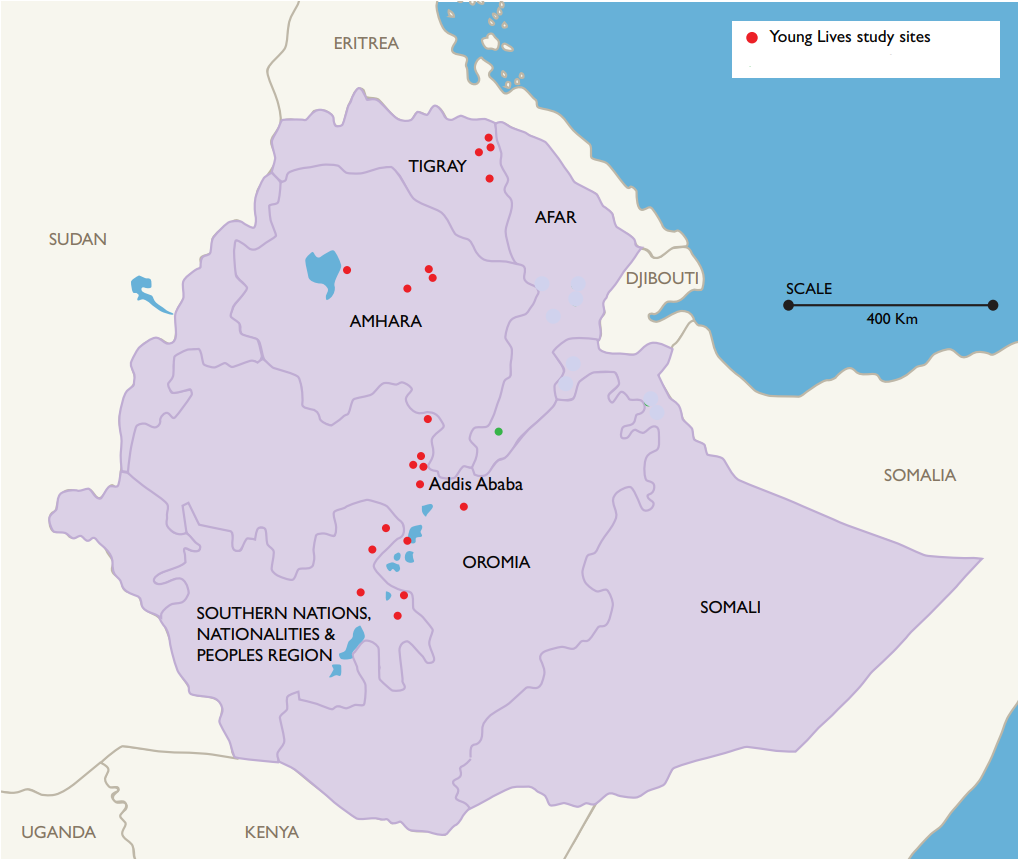
\includegraphics[width=.5\textwidth]{figures/map.png}
\caption*{{\small \textit{Source}: Vujcich, D. (2013). Policy and practice on language of instruction in Ethiopian schools: findings from the Young Lives school survey (Publisher's version). Young Lives. p.~2 (modified).\nocite{Vujcich2013}}}
\end{figure}



\end{document}